\documentclass[10pt]{article}
\usepackage[utf8]{inputenc}

%%% PAGE DIMENSIONS
\usepackage{geometry} % to change the page dimensions
\geometry{a4paper} % or letterpaper (US) or a5paper or....
% \geometry{margin=2in} % for example, change the margins to 2 inches all round
% \geometry{landscape} % set up the page for landscape

\usepackage{graphicx} % support the \includegraphics command and options

%%% PACKAGES
\usepackage{booktabs} % for much better looking tables
\usepackage{array} % for better arrays (eg matrices) in maths
\usepackage{paralist} % very flexible & customisable lists (eg. enumerate/itemize, etc.)
\usepackage{verbatim} % adds environment for commenting out blocks of text & for better verbatim
\usepackage{subfig} % make it possible to include more than one captioned figure/table in a single float
% These packages are all incorporated in the memoir class to one degree or another...

%%% HEADERS & FOOTERS
\usepackage{fancyhdr} % This should be set AFTER setting up the page geometry
\pagestyle{fancy} % options: empty , plain , fancy
\renewcommand{\headrulewidth}{0pt} % customise the layout...
\lhead{}\chead{}\rhead{}
\lfoot{}\cfoot{\thepage}\rfoot{}

%%% SECTION TITLE APPEARANCE
\usepackage{sectsty}
\allsectionsfont{\sffamily\mdseries\upshape} % (See the fntguide.pdf for font help)
% (This matches ConTeXt defaults)

%%% ToC (table of contents) APPEARANCE
\usepackage[nottoc,notlof,notlot]{tocbibind} % Put the bibliography in the ToC
\usepackage[titles,subfigure]{tocloft} % Alter the style of the Table of Contents
\renewcommand{\cftsecfont}{\rmfamily\mdseries\upshape}
\renewcommand{\cftsecpagefont}{\rmfamily\mdseries\upshape} % No bold!



%%% END Article customizations

\usepackage{giorgio_style}

\begin{document}

\begin{titlepage}
\newcommand{\HRule}{\rule{\linewidth}{0.5mm}}
\center 
\textsc{\LARGE Sapienza University of Rome }\\[1.5cm] 
\HRule \\[0.4cm]
{ \huge \textbf {Mining Evolving Topics }}\\[.75cm]
{\Large Web and Social Information Extraction Assignment}\\[0.4cm]
\HRule \\[1.5cm]

\begin{minipage}{0.4\textwidth}
 \large
\emph{Author:}\\[0.5cm]
\Large  Giorgio \textsc{Mariani} 
\end{minipage} \\[3cm]


\includegraphics[width=7.4cm]{logo.png}
\vfill 
\end{titlepage}

%NEW commands
\newcommand{\DSone}{\textbf{DS-1}}
\newcommand{\DStwo}{\textbf{DS-2}}
\newcommand{\set}[1]{#1}
\tableofcontents


%start report
\newpage
\section{Introduction}
This document is a report of the \textbf{Web and Social Information Extraction Course} project.
% TODO give description of input data
The project consists of two correlated tasks that need to be solved:
\begin{description}
\item[Task 1] requires the extraction of topics for each year between 2000 and 2018, included. These topics should be extracted by processing information contained in several keyword co-occurrence graphs (one per year). Diffusion models have to be utilized in order to determine the nodes inside a topic.

\item[Task 2] asks for the tracking and merging of the previously gathered topics throughout the years between 2000 and 2018. The results of this task is a set of time-fused topics.
%\textit{Direct Acyclic Graph} (DAG) mapping topics from one year to topics in the next one.%are twice: a set of topics sequences indicating the evolution of a certain topic over time, and a set of topics obtained by merging the topic information through time. 
\end{description}

\subsection{Technologies}
\paragraph{\textbf{Python Interpreter version 3.7.}}
The Language used in the project is \textbf{Python} version 3.7, this language was chosen mainly due to the availability of specific computation libraries such as \textbf{NumPy} and \textbf{NetworkX}. The flexibility of the language also allows for very fast prototyping, which can help in an project like the one proposed, since different approaches were studied during the project progression.

\paragraph{\textbf{NumPy Module.}} It is one of the fundamental packages for scientific computing with Python. It contains among other things: a powerful N-dimensional array object, tools for integrating C/C++ code, linear algebra functions, Fourier transform, and random number capabilities.

\paragraph{\textbf{NetworkX Module.}} This module is a Python library designed for the creation, manipulation, and analysis of different types of networks. It offers a variety of already implemented graph algorithms, such as PageRank, Betweenness Centrality, etc.
It is [..]

\paragraph{\textbf{igraph-python Module.}}
\textbf{igraph} was also used as graph processing library during the early phase of the project, however due to the lack of certain algorithms and the overall less intuitive interface, this package was abandoned for the simpler \textbf{NetworkX}. It should be said, although, that \textbf{igraph} achieved better performance in the various tasks.


\subsection{Data}
The datasets used in the project are two: one containing information about keywords co-occurrence, and one containing co-authorship data. Both datasets are domain-specific and contain entries associated only to machine-learning related articles and papers. 

\paragraph{\textbf{Dataset \DSone}.}
As mentioned, the first dataset (denoted  as \DSone{}) contains information about keyword co-occurrence throughout some intervals of years, including between 2000 and 2018. Formally, it contains rows with the following structure:
\begin{center}
\newcommand{\TAB}{\textless tab\textgreater}
\textbf{y} \TAB{} \textbf{k\textsubscript{i}} \TAB{} \textbf{k\textsubscript{j}} \TAB{} [\textbf{a\textsubscript{0}}:$n_0$ ,..., \textbf{a\textsubscript{m}}:$n_m$]
\end{center}
with \textbf{k\textsubscript{i}} and \textbf{k\textsubscript{j}} two co-occurring keywords, \textbf{y} the year in which they co-occur, while $n_k$ is the number of articles published by author \textbf{a\textsubscript{k}} containing both \textbf{k\textsubscript{i}} and \textbf{k\textsubscript{j}}.
Therefore, this dataset implicitly defines a number of graphs, one per year, describing co-occurrence relationships. %The author information is also used to calculate weights over these co-occurrences (see \cref{sec:weights}).



\paragraph{\textbf{Dataset \DStwo}.}
This dataset stores information about co-authorship between  authors during several years, including the time-interval from 2000 to 2018.  Rows in the dataset are defined as  
\begin{center}
\newcommand{\TAB}{\textless tab\textgreater}
\textbf{y} \TAB{} \textbf{a\textsubscript i} \TAB{} \textbf{a\textsubscript j} \TAB{} \textbf{n}
\end{center}
with \textbf{y} the co-authorship year, \textbf{a\textsubscript{i}} and \textbf{a\textsubscript{j}} the collaborating authors, and \textbf{n} the number of  collaborations between   \textbf{a\textsubscript{i}} and \textbf{a\textsubscript{j}} within the year.\\
Again, this dataset can be seen as a sequence of graphs (one per year), having as nodes authors and as edge information about the co-authorship relation.
 
\newpage
\section{Diffusion Models}
\subsection{Linear Threshold Model}\label{sec:ltm}
The \textit{linear threshold model} \cite{diffusion} is a diffusion model, which are a class of models sometimes adopted in order to represent the rate of diffusion of an information in a given network.\\
Differently from simpler models like the \textit{tipping model} and the \textit{SIR model}, the linear threshold makes use of information between edges, making it more compelling for this project; Specifically, in the linear threshold model, each directed edge $(u,v) \in E$ has associated a non-negative weight $w_{u,v}$, with the additional constraint that for any node $v\in V$, the total in-neighbor sum\footnote{Throughout this document, we refer to the \textit{in-neighbor sum} of a node as the sum of all its incoming edges weights.} must be less than or equal to one
\begin{equation}\label{eq:linear_threshold_constraint} 
    \sum_{u\in \InNeighbours (v)} w_{u,v}\le 1
\end{equation}
in order to be consistent.

Given a \textit{Social Network}, represented by the graph $G=(\Vertices,\Edges)$ (with $|\Vertices|=n$ and $|\Edges|=m$), the linear threshold model computes a set of nodes that might\footnote{Since the algorithm is randomized, this will change depending on the execution.} be influenced by an initial set of source nodes (referred to as $A_\theta^{(0)}$). The process works by first assigning (uniformly at random) to each vertex $v$ a threshold value $\theta_v\in(0,1]$, then it proceeds at iterations, where in iteration $i$, it expands the set of currently active nodes (indicated by $A_\theta^{(i)}$) until convergence is reached.  The active nodes at iteration $i$ are update through  the following recurrent equation:
$$
A^{(i+1)}_{\theta}=A^{(i)}_{\theta}\cup{}\left\{v\in \Vertices : \sum_{u\in\InNeighbours{}(v)\cap A^{(i)}_{\theta}} w_{u,v}\ge \theta_v\right\}
$$
The set of active nodes $A^{(i)}_\theta$ is said to have reached convergence if and only if $A_\theta^{(i)} = A_\theta^{(i+1)}$.

\subsection{Average Linear Threshold}\label{sec:altm}
As previously stated, the linear threshold model is a randomized process with the output varying depending on the threshold assignments; in order to reduce the output sensitivity, instead of giving a boolean output for each node $v$ (\ie{} the node was/wasn't influenced), it is possible to execute the algorithm a number of times\footnote{For this project, the algorithm is invoked 12 times  in order to compute the relative frequencies.} ($n$) and using the average infection rate $\alpha_v\in[0,1]$ as output:
\begin{equation}
\alpha_v = \frac{1}{n}\sum_{i=0}^{n} b_{v}^{(i)}
\end{equation}
with $b_{v}^{(i)}\in \{0,1\}$ indicating the result of linear threshold during trial $i$.


\paragraph{\textbf{Probabilistic interpretation.}}
This value can be seen as an estimator for the probability of infection of the node $v$, if the set of nodes $S$ is the infection source:
$$P\{\text{$v$ is infected $|$ $S$ as source}\}=\alpha_{v,S}$$
%This probability is estimated through the relative frequency of infection; the linear threshold algorithm is applied a number of times (using $S$ as source set), then the probability of infection of $v$ is estimated as the  division between the number of times $v$ was infected by the total number of trials: 
%\begin{equation}\label{eq:infection_prob}
%    \hat P\{\text{$v$ is infected $|$ $S$ as source}\} = \frac{\text{num. of trials in which $v$ was infected}}{\text{number of trials}}
%\end{equation}

\paragraph{\textbf{Fuzzy Set interpretation.}} It is possible to interpret the value $\alpha$  as  how much the node $v$ is contained in the set of nodes infected by the source set $S$. So if a fuzzy set \cite{fuzzy} is used to describe the nodes infected by $S$, then $\alpha_{v,S}$ can represent its membership function:
\begin{definition}
A \textit{Fuzzy Set} $\Fuzzy{F}$ in $X$ is a set of ordered pairs:
$$
\Fuzzy{F} = \left\{(x, \mu_{\Fuzzy{F}}(x)): x\in X \right\}
$$
The function $\mu_{\Fuzzy{F}}:X \rightarrow{} [0,1]$ is called \textit{membership function}, and describes how much a given element $x$ belongs to the set $\Fuzzy{F}$.
\end{definition}
Using this definition, it is possible to define the set of nodes influenced by the source $S$ as the fuzzy set:
$$\Fuzzy{S} = \Big\{(v, \mu_{\Fuzzy{S}}(v)): v\in V, \mu_{\Fuzzy{S}}(v) = \alpha_{v,S}\Big\}$$


\newcommand{\Visited}{\mathrm{visited}}
\newcommand{\Output}{\mathrm{result}}
\begin{algorithm}
	\caption{Linear Threshold Model}
\begin{algorithmic}[1]
	\Require{graph $G$, with nodes $\Vertices(G)$.}
	\Require{source node $s\in \Vertices(G)$, in which the algorithm starts diffusing influence.}
	\Statex{}
	\Procedure{linear\textunderscore{}threshold\textunderscore{}model}{$G$, $s$, $\theta$}
	\State $\Visited \leftarrow$ array with size $|\Vertices(G)|$ containing all zeros entries.
	\State $\Visited[s] \leftarrow 1$
	\State {$Q \leftarrow$ new queue containing only $s$.}
	\While{$Q$ is not empty}
		\State $v \leftarrow$ dequeue($Q$)
		\For{ $u \in \OutNeighbours(v)$}
			\If {$\Visited[u] < {\theta}_{u}$}
				\State $\Visited[u] \leftarrow \Visited[u] + w_{v, u}$
				\If {$\Visited[u] \ge \Vec{\theta}_{u}$}
					\State {enqueue($Q$, $u$)}
				\EndIf
			\EndIf
		\EndFor
	\EndWhile
	\State $\Output \leftarrow$ array with size $|\Vertices(G)|$ containing all zeros entries.
	\For{$u\in \Vertices(G)$}
		\State $\Output[u] \leftarrow \begin{cases} 1 &\text{if } \Visited[u] \ge \theta_{u}\\
		0 &\text{otherwise}
		\end{cases} $
	\EndFor
	\State{\Return $\Output$}
	\EndProcedure
\end{algorithmic}
\end{algorithm}
\newpage
\section{Task 1}

% LINK https://towardsdatascience.com/ways-to-detect-and-remove-the-outliers-404d16608dba
\subsection{Edge Weight Selection}\label{sec:weights}
The edge-weights were selected using information from  both datasets \DSone{} and \DStwo{}; after selection  these weights are then normalized in order to better be exploited by the linear threshold model. The formula used to compute these edge weights, prior the normalization step, is quite intuitive and can be described as the sum of the number of articles containing the both keywords $k_1$ and $k_2$, weighted by the rank of the articles' authors. The rank is obtained by computing the \textit{pagerank} of the author graph of the respective year.\\
The formulation of these pre-normalization edge weights (for example, between keywords $k_1$ and $k_2$) is given by
\begin{equation}\label{eq:weight_prenorm}
w_{k_1,k_2}=\sum_{a_i} \mathrm{rank}(a_i)\cdot \mathrm{count}_{k_1,k_2}(a_i)    
\end{equation}
where $a_i$ varies over the set of all authors, ${rank}(a)$ is the pagerank of author $a$, and ${count}_{k_1, k_2}(a)$ is the number of articles having as author $a$ and containing both $k_1$ and $k_2$.
The pagerank of an author (for a given year $y$) is obtained by computing the pagerank of co-authorship graph for the respective year.

% TODO add outlier detection
\paragraph{\textbf{Outlier Correction.}} One problem that was encountered during the first phase of the project was the presence of outlier edge-weights. Indeed, the weights computed using the \cref{eq:weight_prenorm} can be heavily unbalanced (as can be seen in  \cref{fig:weight_prenorm}), which caused a number of problems when trying to apply the linear threshold algorithm. This problem was approached by using a simple outlier correction strategy; using the \textit{z-score} of the edge-weight distribution, clamping elements with a \textit{z-score} higher than three.

  \begin{figure}[h!]
     \centering
     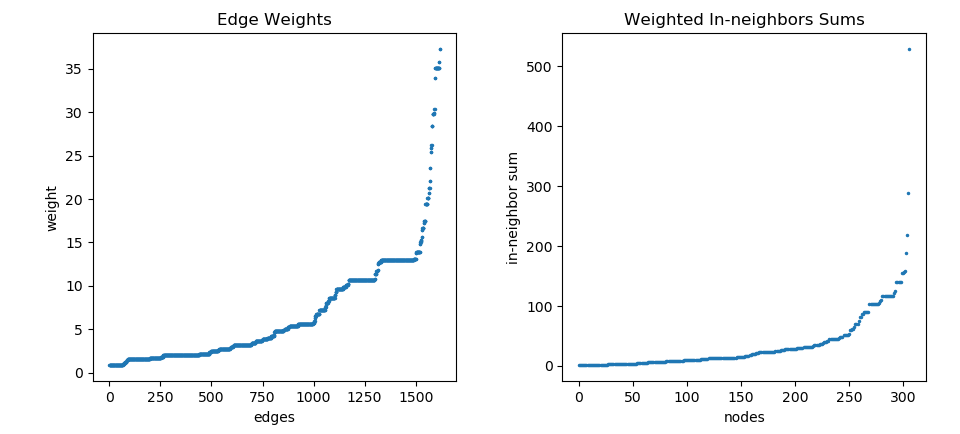
\includegraphics[width=\textwidth]{img/prenorm.png}
     \caption{Graphs showing the distribution of the edge-weights and of the in-neighbors sums \textbf{before} the normalization step.}
     \label{fig:weight_prenorm}
 \end{figure}
 
\paragraph{\textbf{Normalization.}}
As previously mentioned, in order to use these calculated edge-weights with the linear threshold algorithm (see \cref{sec:ltm}), a normalization step is necessary. 
 Indeed, remember that the in-neighbors sums must be less then or equal to one for each node in the input graph, which may not be true for the weights computed using \cref{eq:weight_prenorm}. Another problem is that if the in-coming weights of a node are too small then they will not be able infect it, hence blocking the diffusion process.\\ 
 A number of possible strategies can be used in order to avoid these situation, in particular, for this project three types were considered:
 \begin{itemize}
     \item The simplest normalization strategy is to scale all the weights $w_{u,v}$ such that  \cref{eq:linear_threshold_constraint} must be valid for all nodes $u$. This can be achieved by dividing all the weights by the maximum in-neighbors sum. That is,
     \[\hat w_{v,u} = \frac{w_{v,u}}{\displaystyle \vphantom{\bigg(} \max_{y} \Big\{\sum_{x\in \InNeighbours(y)} w_{x,y}\Big\}}\]
     This normalization, however, caused the edges' weights to be far too unbalanced, favouring nodes with a high number of in-neighbours, and virtually never activating nodes with fewer incoming edges.
     \item Another strategy initially adopted consisted in forcing the sum of all the in-coming neighbors of all nodes to be $1$. This can be accomplished by locally scaling each weight with the formula
     \[
     \hat w_{v,u} =\frac{w_{v,u}}{\displaystyle \sum_{v'\in \InNeighbours(u)}w_{v',u}}
     \]
     The major drawback of this approach is that nodes with a single incoming vertex  are always activated with their incoming neighbor. More generally, nodes with a low number of in-coming neighbours are favoured while using this normalization approach.
     \item The final normalization strategy, which is the one actually adopted in this project, consists in employing a logarithmic balancing of the in-neighbors summations.
     \[
     \hat w_{v,u} = \frac{w_{v,u}}{\vphantom{\bigg(} \displaystyle \log\Big( 1 + \sum_{x\in \InNeighbours(u)}w_{x,u}\Big)}\cdot z
     \]
     with $z$ a normalization factor such that 
     \[\max_{u}\Big\{ \sum_{v\in \InNeighbours{u}}\hat w_{v,u} \Big\} = 1\]
     The use of the logarithm allows the in-neighbors sums to be well distributed, so that nodes with less nodes can be activated. This method proved to create topics that are somewhat balanced. It is possible to see the difference between before and after this normalization process respectively in \cref{fig:weight_prenorm} and \cref{fig:weight_afternorm}.
 \end{itemize}
 
\begin{figure}[h!]
     \centering
     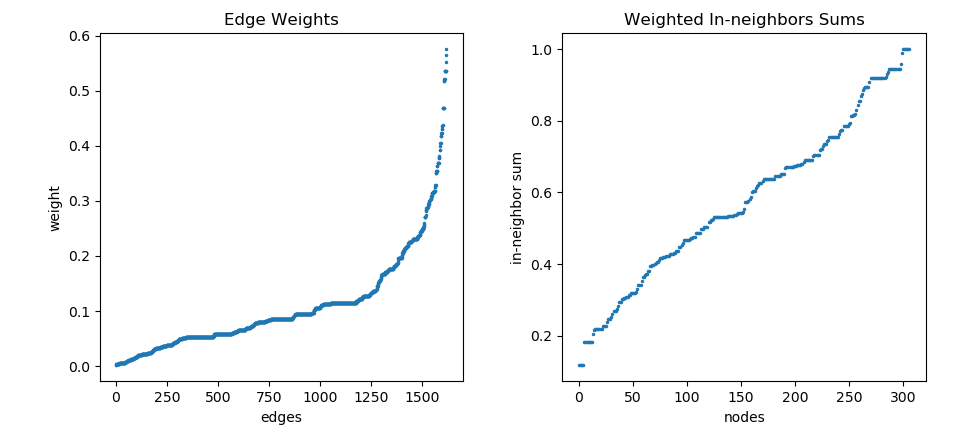
\includegraphics[width=\textwidth]{img/afternorm.png}
  \caption{Graphs showing the distribution of the edge-weights and of the in-neighbors sums \textbf{after} the normalization step.}
  \label{fig:weight_afternorm}
 \end{figure}
  

 
\subsection{Topicness}\label{subsec:topicness}
Following the project's specification, topics are estimated by applying the linear threshold model over some source nodes, which have to be extracted using a metric to define, \ie{} pagerank, cluster-coefficient, \etc{}. During development, different such metrics were tested and refined. At first, the pagerank was utilized in order to pick the best candidates. However, two major problems resulted from using pagerank: a strong bias towards hubs (which are not necessarily good topic sources), and a problem with the \enquote{picking} strategy, since simply taking the nodes with highest value will take nodes most likely near to the core of the graph's main component.\\
To solve the first problem a combination of metrics were utilized, specifically, two others besides pagerank: \textit{Local Cluster Coefficient}, and \textit{Betweenness Centrality}. The local cluster coefficient of a node indicates how much the neighbors of a node are interconnected with each-others; it is intuitive that good topics sources have an higher cluster coefficient than normal nodes. For un-directed un-weighted graphs, the cluster coefficient of $u$ is described by
\[
\mathrm{cluster\ coefficient}(u) = \frac{2\Big|\Big\{\{v,w\}\in \Edges:v\in\Neighbours(u), w\in\Neighbours(u)\Big\}\Big|}{d_u\cdot(d_u - 1)}
\]
However, the directed weighted variant described in \cite{clustering} (implemented by \textbf{NetworkX}) was used for this project.

It was possible to improve the initial pagerank estimation by adding the information found in the cluster coefficient. This was done by using, instead of standard pagerank, the \textit{personalized-pagerank} algorithm, with personalization vector the cluster-coefficient (after being appropriately scaled to a probability distribution).
The difference, using as dumping factor $0.8$, can be seen in \cref{fig:pagerank_comparison}.
\begin{figure}[h!]
		\centering
		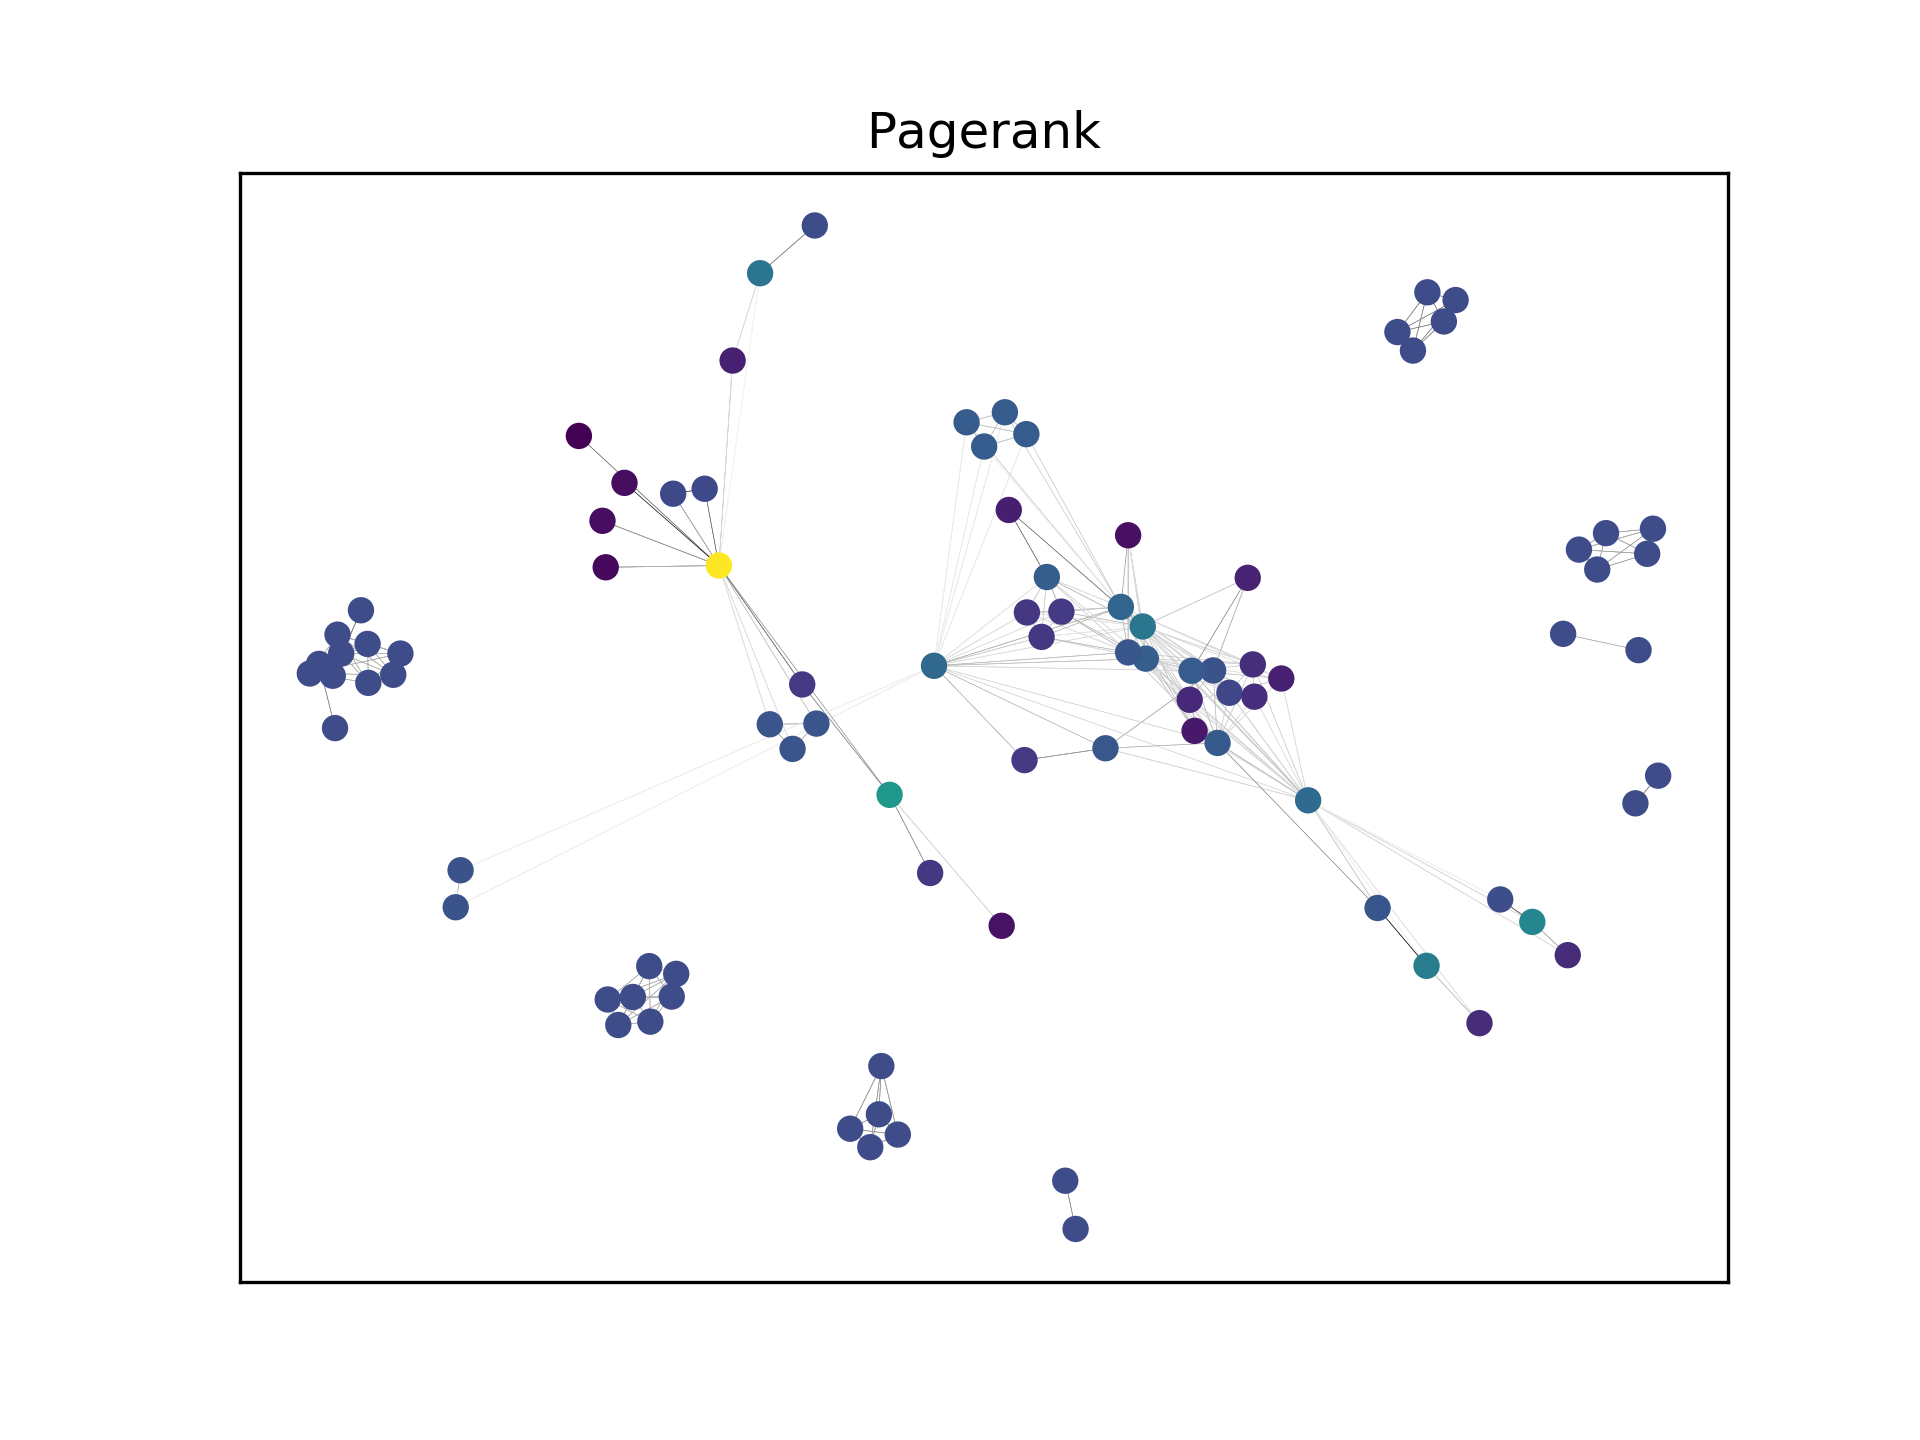
\includegraphics[width=.495\textwidth]{img/pr.png}
		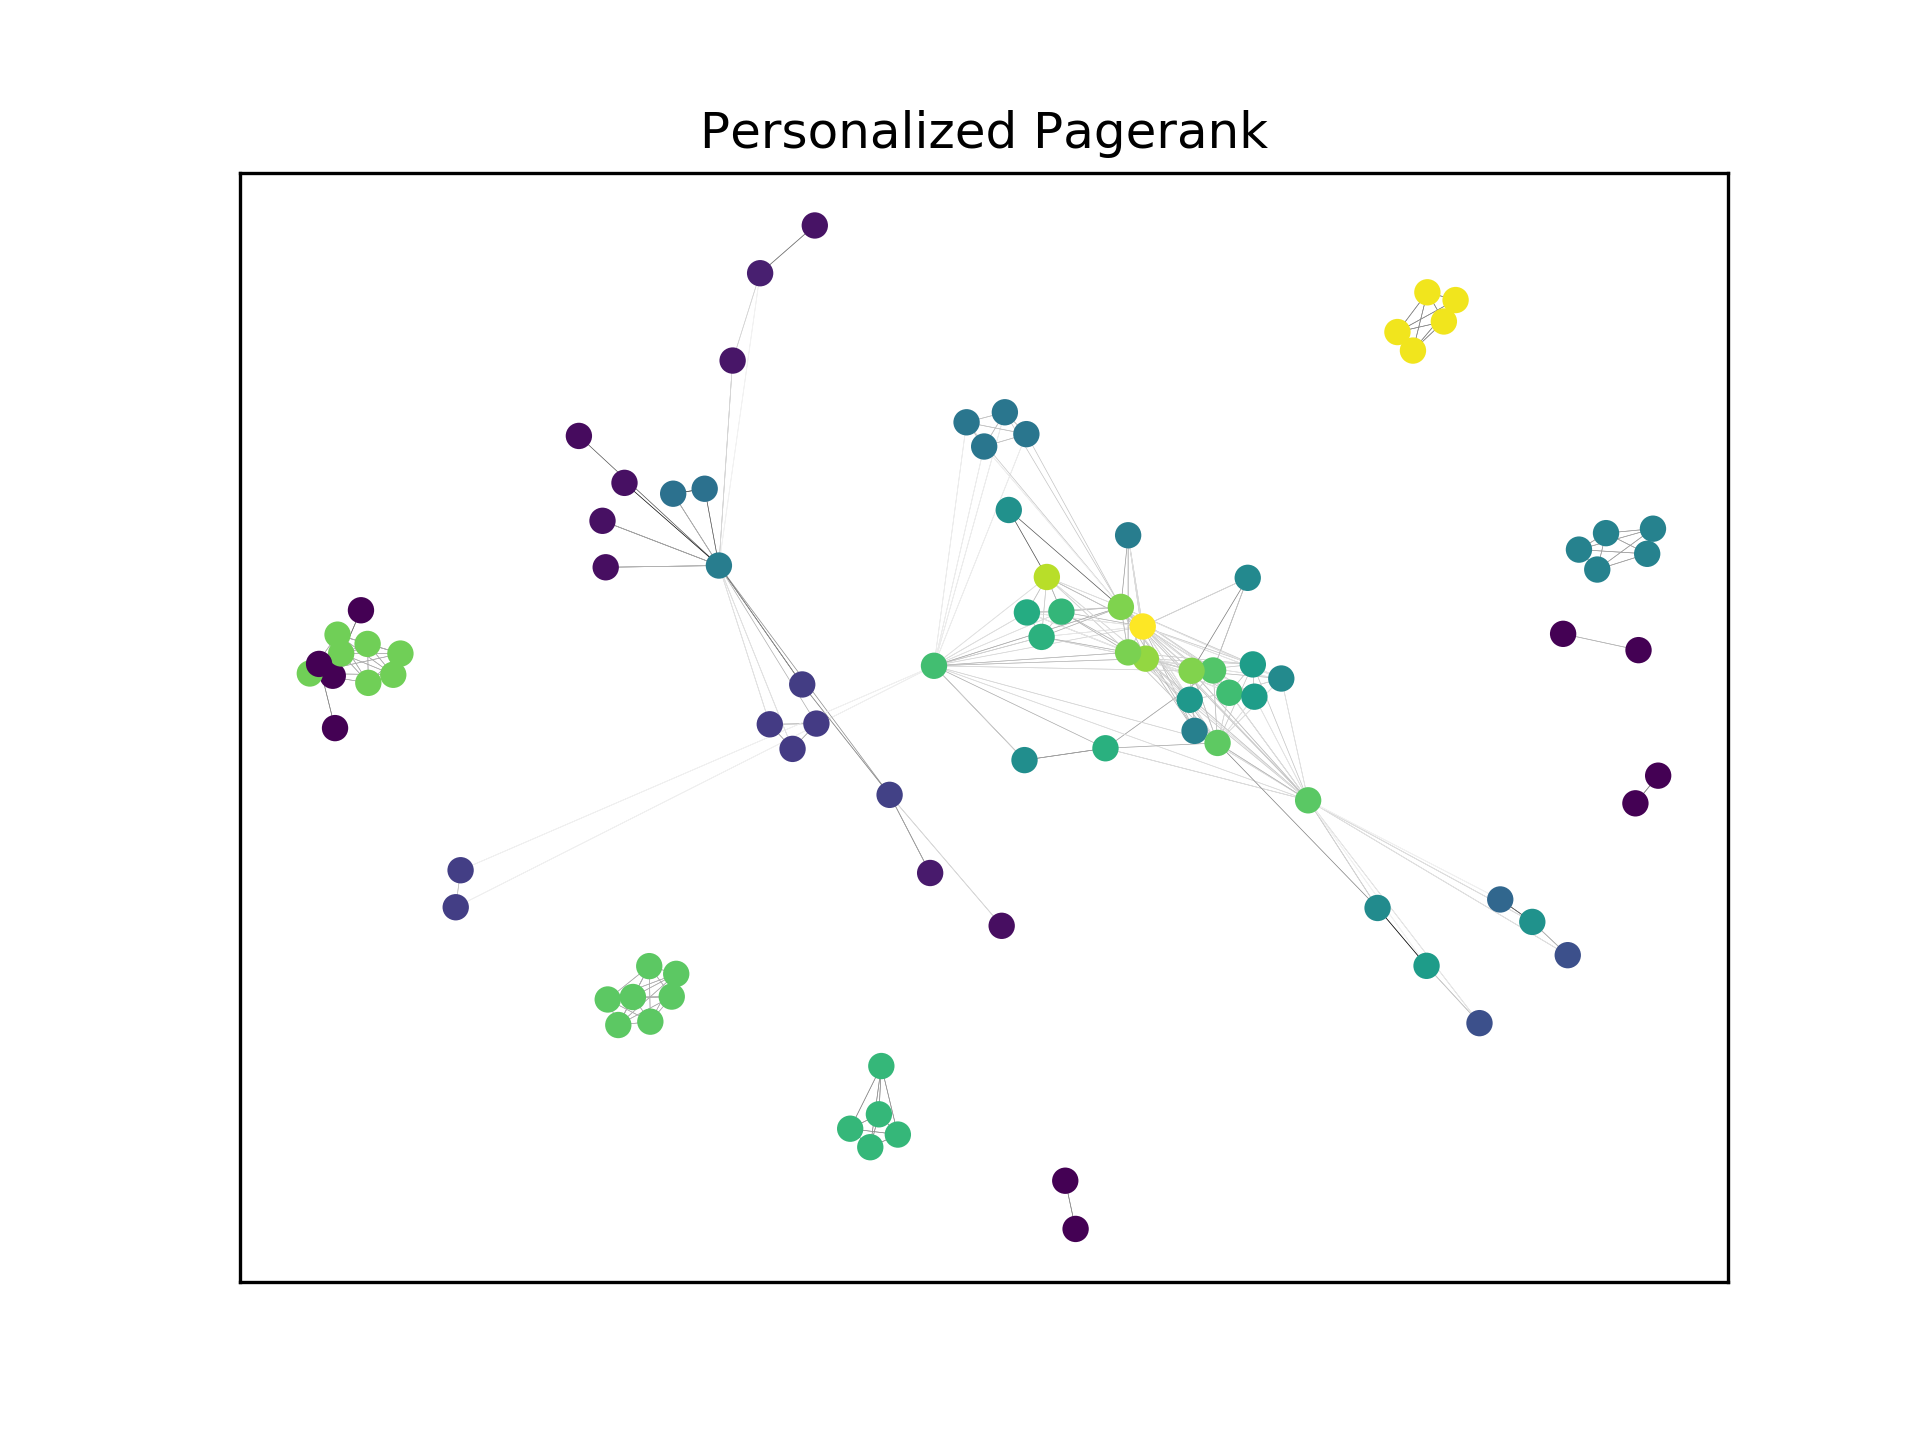
\includegraphics[width=.495\textwidth]{img/ppr.png}\\
		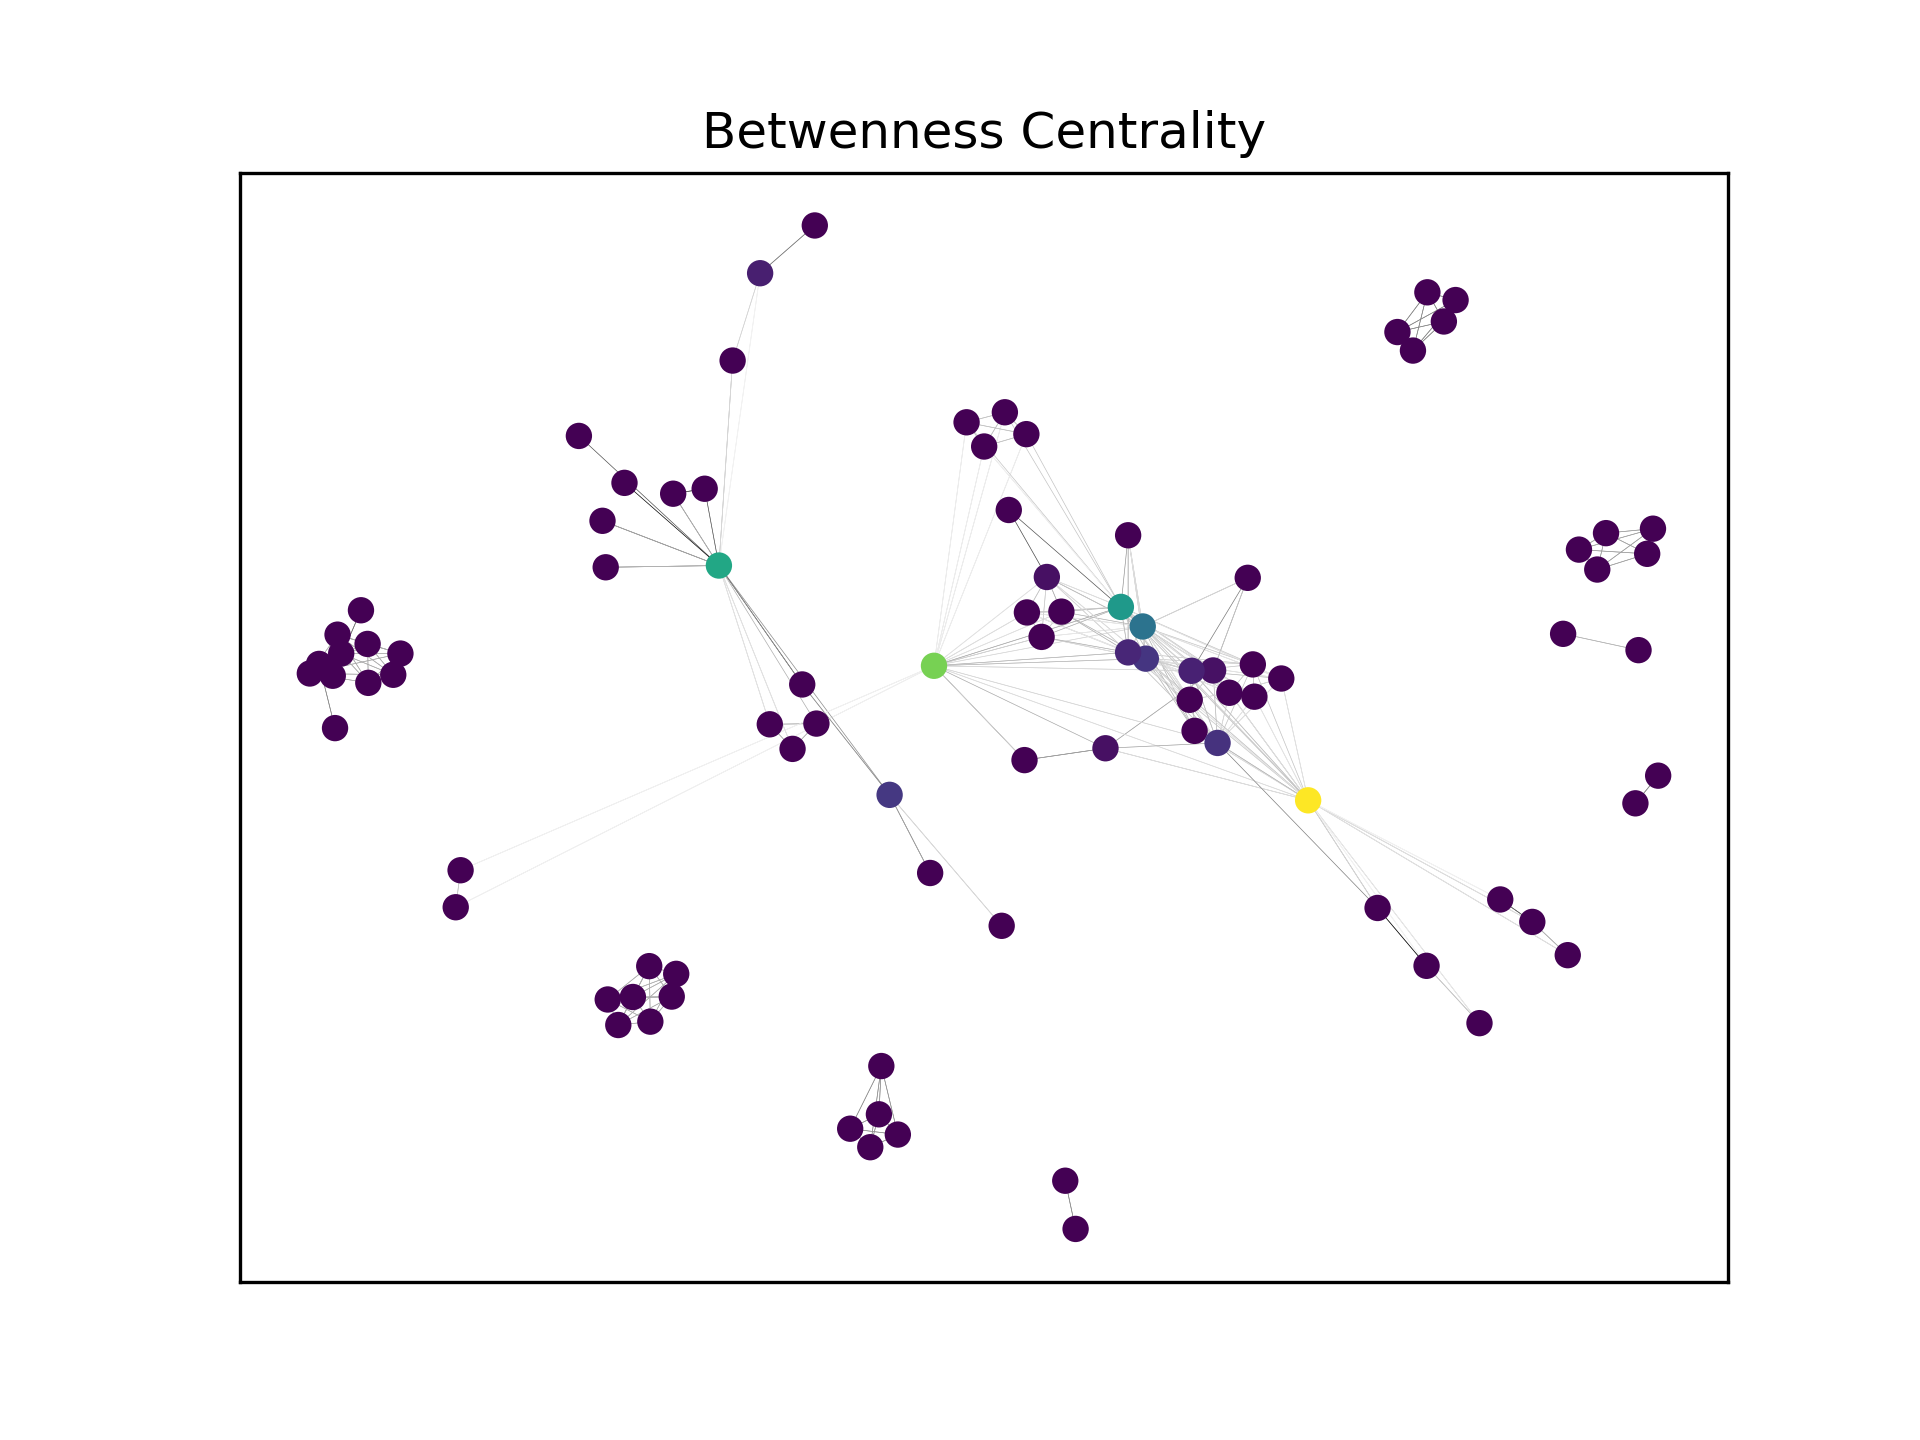
\includegraphics[width=.495\textwidth]{img/bc.png}
		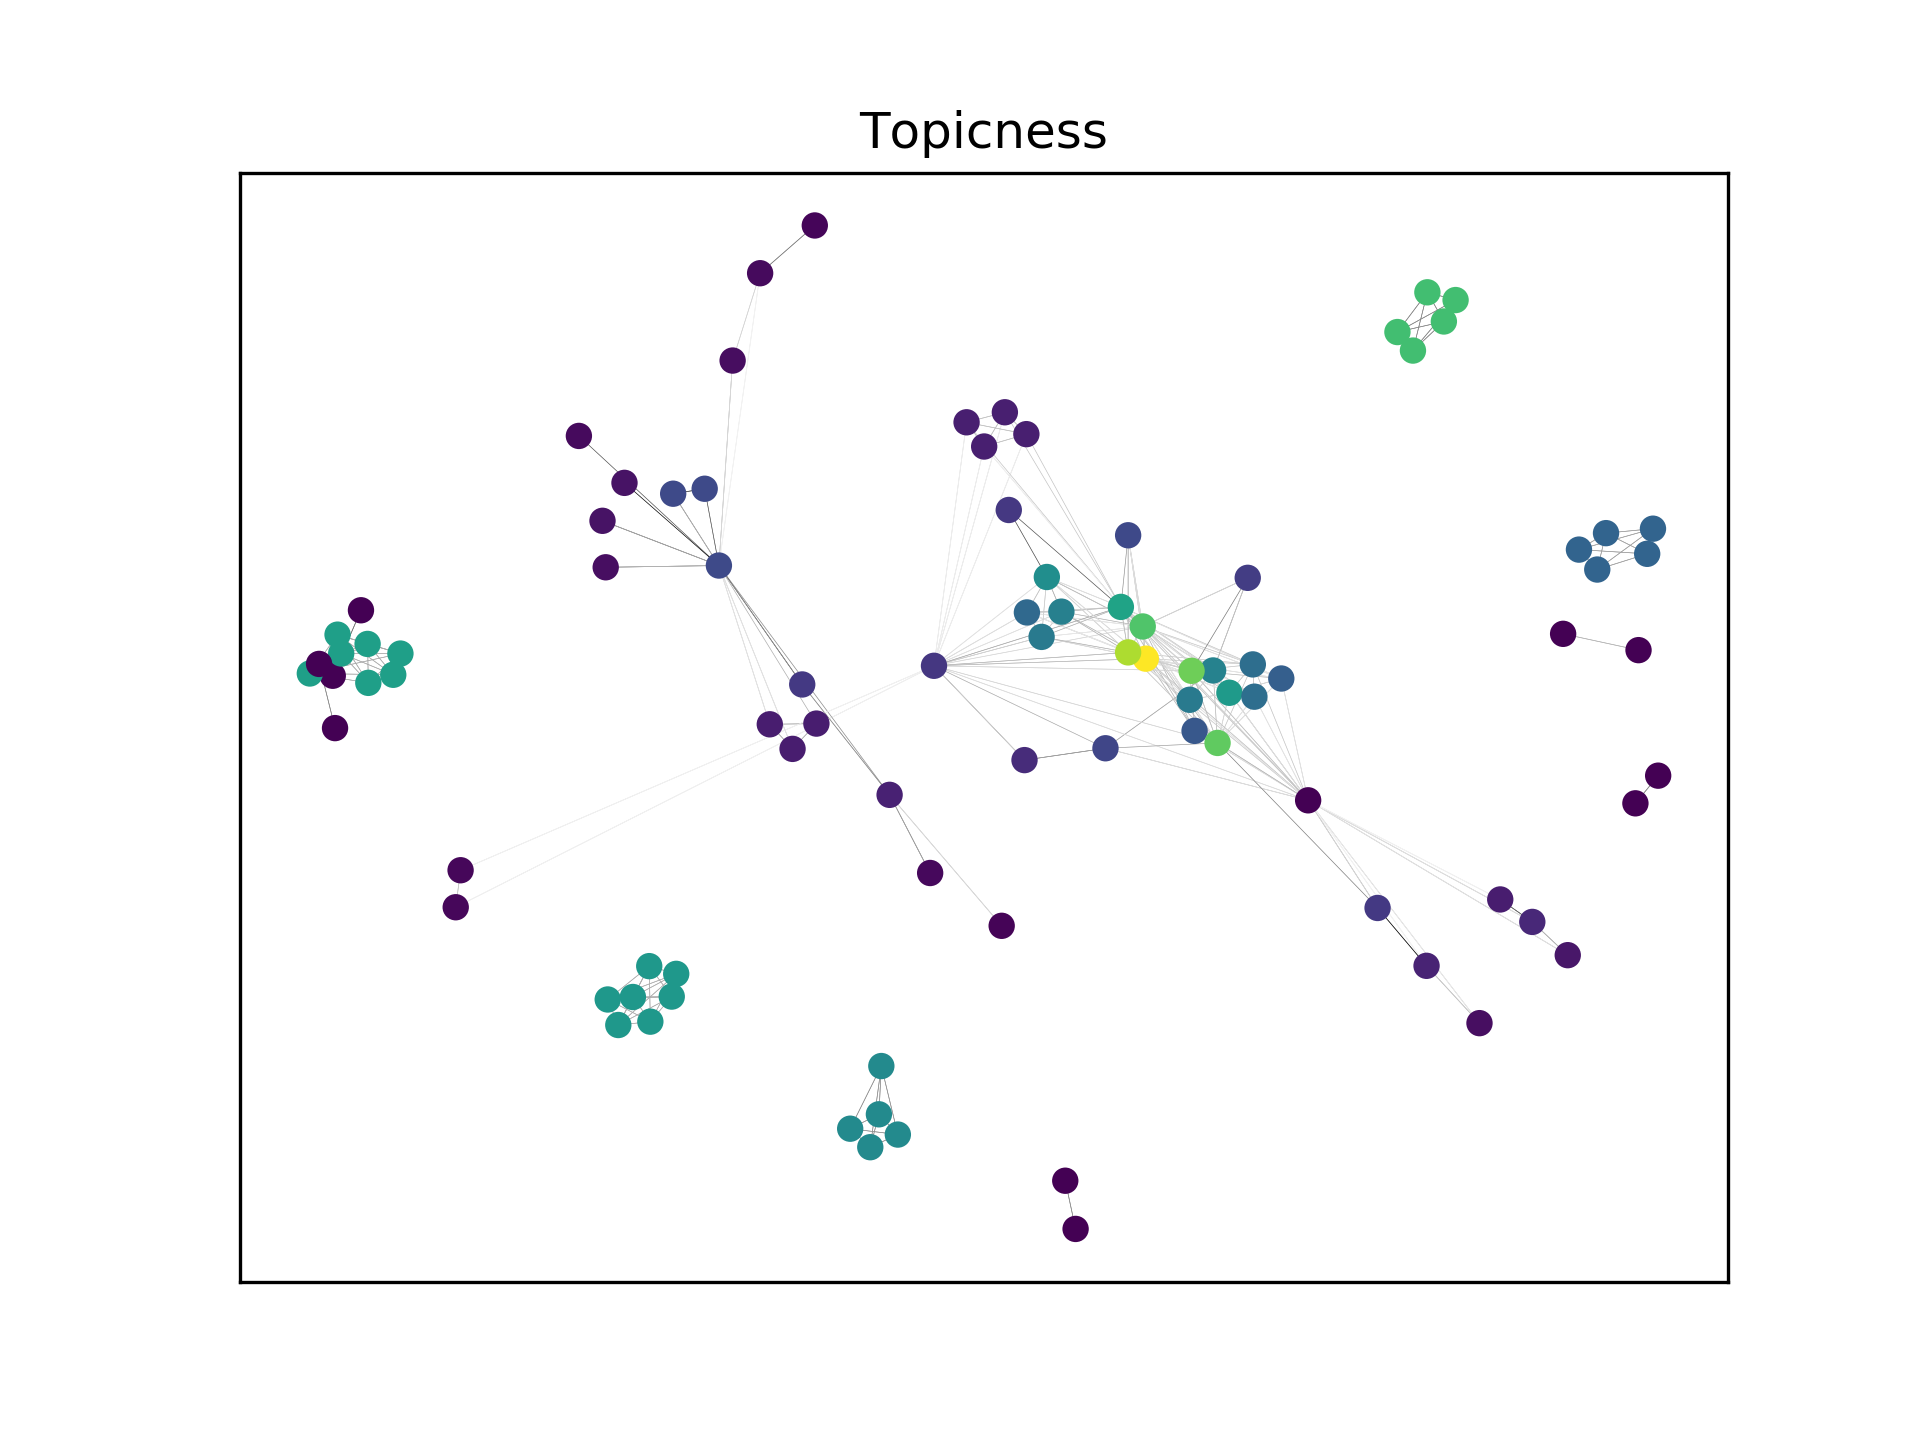
\includegraphics[width=.495\textwidth]{img/tp.png}
		\caption{Comparison between standard Pagerank, Personalized Pagerank (using local Cluster-Coefficient), Betwenness Centrality, and Topicness.}
		\label{fig:pagerank_comparison}
\end{figure}
Despite improving on the initial function, the personalized-pagerank remained yet too inclined towards really big hubs; in order to reduce this bias a new metric was introduced, the aforementioned betweenness centrality. The personalized pagerank values are scaled down proportionally to their betweenness score, which was found to be impacting only nodes that represents big \enquote{hubs} in the graph. The resulting metric, denoted as \textit{topicness}, is hence given by the equation:  
\begin{equation}\label{eq:topicness}
\mathrm{topicness}(u) = \mathrm{personalized\text{-}pagerank}(u)\cdot \Big(1-\mathrm{betweenness}(u)\Big) 
\end{equation}
for each $u\in \Vertices$. 

\subsection{Topic Extraction} Topics are extracted using an iterative method: at each iteration the node associated to the global maximum value\footnote{If there is more then one maximum, then the node is arbitrarily chosen  between those.} of the topicness function is  extracted; after that, the influence of said node is used to update the topicness "surface", in order to obtain a different maximum in the next iteration (see \cref{alg:topic_extraction}).
\newcommand{\Topicness}{\mathop{\texttt{topicness}}}
\begin{algorithm}[H]
\caption{Topic Extraction}\label{alg:topic_extraction}
\begin{algorithmic}[1]
    \Require{$\mathrm{graph}$, keyword co-occurrence graph for a specific year, with $n$ vertices.}
    \Require{$\Topicness$, array of size $n$, indicating topicness for each node.}

    \Statex
    \Procedure{topic\textunderscore{}extraction}{$\mathrm{graph}$, $\Topicness$}
    \State{$S\leftarrow \emptyset$}
	\While{$\exists x: \Topicness[x] > 0$}
	   \State $\mathrm{maxnode} \leftarrow \mathrm{argmax}_{v}\{\mathrm{topicness}[v]\}$ 
	   \State $\mathrm{topic} \leftarrow \texttt{\color{AlgProcedureColor}node\textunderscore{}influence}(\mathrm{graph}, \mathrm{maxnode})$\Comment{$topic$ is an indicator array.}
	   \For{$u= 1 \dots n$}
	    \State $\Topicness[u] \leftarrow \Topicness[u]\cdot(1 - \mathrm{topic}[u])$
	   \EndFor
	   \State{$S\leftarrow S\cup \{\mathrm{maxnode}\}$}
	\EndWhile
    \State{\Return{S}}
	\EndProcedure
\end{algorithmic}
\end{algorithm}
\paragraph{\textbf{Node influence.}} The \texttt{\color{AlgProcedureColor}node\textunderscore{}influence} is computed using the average linear threshold algorithm, as described in \cref{sec:altm}; hence the variable $\mathrm{topic}$ is a vector of size $n$ with values between $0$ and $1$, indicating how much a certain node belongs to the topic identified by the chosen source node. During the project development two methodologies were tested for choosing the value of the topic vector:
\begin{description}
\item[Fuzzy:] At first, the topics were considered as fuzzy topics, using the output of the average linear threshold as description of the topic.
However, this caused some problems during the tracking phase, as topics tended to be too unbalanced towards the source (whose membership value is always one).
\item[Crisp:] After the problems induced by the fuzzy sets during the second task, it was decided to use standard (\ie{} crispy) sets in order to describe topics. Of course, this requires a \textit{defuzzification} procedure, which may loose information.
\end{description}



\subsection{Defuzzification of topics}
Fuzzy set theory uses several strategies in order to converted fuzzy sets to standard sets. These may range from mean based techniques, to more sophisticated algorithms. In our case, the algorithm is fairly simple; the $k=6$ nodes with higher membership values (only if they are different from zero) are considered as the crisp representation of the topic. More formally, if $x$ is in the defuzzification $S$ of $\Fuzzy{F}$, then 
$$
    x\in S \implies \begin{cases}
    \forall y\not\in S: \mu_{\Fuzzy{F}}(x) \ge \mu_{\Fuzzy{F}}(y)\\
    \mu_{\Fuzzy{F}}(x) > 0
    \end{cases}
$$
and the size of $S$ must be less then or equal to $k$ (\ie{} $|S| \le k$).
This is done in order to prevent the creation of topics  that are either too big or too small, and six was experimentally a good number for topic size. The conversion procedure can be seen in \cref{alg:defuzzification}.
\begin{algorithm}
\caption{Defuzzification}\label{alg:defuzzification}
\begin{algorithmic}[1]
    \Require{$F$, sequence of length $n$ and containing pairs $(x,\mu_{\Fuzzy{F}}(x))$. This object represents the fuzzy set $\Fuzzy{F}$}
    \Statex
    \Procedure{defuzzification}{$F$, $k$}
        \State{} $ S \leftarrow \emptyset$ 
        \State{} Sort array $F$ w.r.t. membership values.
        \For{$i= n-k \dots n$}
        \State{} $(x,\mu_{\Fuzzy{F}}(x))\leftarrow F[i]$
        \If{$\mu_{\Fuzzy{F}}(x) > 0$}
         $S\leftarrow S \cup \{x\}$
        \EndIf
	\EndFor
	\State \Return{S}
	\EndProcedure
\end{algorithmic}
\end{algorithm}




\newpage
\newpage
\newcommand{\CandidateChain}{\texttt{\color{AlgProcedureColor}candidate\textunderscore{}chain} }
\section{Task2}
During the second task,  the topics extracted in \textbf{Task 1}  are tracked throughout the years and fused together. The set of years to be merged  is indicated by the sequence $\mathcal Y = \{y_i\}_{i=0..18}$.
Two approaches were tested for solving this task:
\begin{itemize}
\item In the first method, topics between adjacent years are linked together, creating then a \textit{direct acyclic graph} of the topics. From this graph are extracted $K=20$ paths, representing the topic evolution. These are then merged in order to represent the final fused topics.
\item The second approach makes use of more information, and uses the similarity of each pair of topics between all the years in $\mathcal Y$. Using this similarity (after being appropriately weighted) chains of topics are computed using a greedy approach. Similarly to the previous approach, these chains are then merged together in order to create the fused topics.
\end{itemize}

\subsection{Keyword Similarity}\label{sec:keyword_similarity}
In order to determine if two topics are related, a metric describing the similarity between two keywords is necessary. This may be useful when trying assess the similarity between topics, especially if said topics do not share a great number of words, but have a lot of similar words in common. The keyword similarities considered for the project are two:
\begin{description}
	\item[Exact Match:] this is a rather simple similarity function, mapping to 1 only pairs of keywords represented by the same exact character sequence. This is a very conservative metric, with high precision but low recall.
	$$
	\KeywordScore(w_1,w_2) = \begin{cases}
	1 & \text{if $w_1 = w_2$}\\
	0 & \text{otherwise}
	\end{cases}
	$$
	\item[Jaccard Similarity:] the similarity between two keywords  is computed  using their \textit{bag-of-words} representation; each keyword is seen as a sequence of smaller words (using white-spaces as delimiter), which are then compared utilizing the \textit{Jaccard Similarity}.\\
	For example consider the keywords: \textbf{\enquote{brown fox}}, and \textbf{\enquote{quick fox}}, the estimated similarity score is given by 
	$$
	\KeywordScore(\textbf{\enquote{brown fox}}, \textbf{\enquote{quick fox}})  = %
	\frac{|\{\textbf{\enquote{fox}}\}|}{|\{\textbf{\enquote{brown}}, \textbf{\enquote{quick}}, \textbf{\enquote{fox}}\}|}= \frac{1}{3}
	$$
	This similarity suffers the opposite problem, since it may give an higher similarity value then it  should, particularly if frequent words are in both keywords.
\end{description}
\subsection{Topic-Pairs Score}\label{sec:topic_score}
The keyword similarity information described in the previous section is then utilized in order to associate topics from different years. This is performed using a score function, and later on using said score to create a relation between nodes in different years. 
% TODO add a simple matrix as example
During the project development, several score-functions were tested, the main one were:
\begin{description}
	\item[Jaccard Similarity:] the jaccard similarity was also used for topics scoring, using the keyword sets associated to each topic. The jaccard score seems to be a simple but effective score, however, it suffers one major drawback: it is not possible to exploit the jaccard keyword similarity previously described in \cref{sec:keyword_similarity}. %and it requires topic to be a crisp set, and does not generalize to fuzzy ones (however, this is less problematic since crisp topics were mostly used in the project).
	$$\TopicScore(T_i,T_j) = \frac{|T_i\cap T_j|}{|T_i \cup T_j|}$$
	\item[Fuzzy Similarity] this similarity was an attempt at a generalization of the  jaccard similarity, while adapting fuzzy topics and exploiting the keyword similarities described before.
	Let $\Fuzzy{T_1}$ and $\Fuzzy{T_2}$ be two fuzzy topics (with respective membership functions $\mu_{\Fuzzy{T_i}}$ and $\mu_{\Fuzzy{T_j}}$)
	\begin{gather*}
		\mathbb I(\Fuzzy T_i,\Fuzzy T_j) = \Membership{\Fuzzy{T_i}}(w_1)\cdot \Membership{\Fuzzy{T_j}}(w_2)\cdot \KeywordScore(w_1,w_2)\\
		\mathbb U(\Fuzzy T_i,\Fuzzy T_j) = \sum_{w_1,w_2}\Membership{\Fuzzy{T_i}}(w_1)\cdot \KeywordScore(w_1,w_2) +  \sum_{w_1,w_2}\Membership{\Fuzzy{T_j}}(w_2)\cdot \KeywordScore(w_1,w_2) - \mathbb I(\Fuzzy T_i,\Fuzzy T_j)
	\end{gather*}
	$$
	\TopicScore(\Fuzzy{T_i}, \Fuzzy{T_j}) = \frac{\displaystyle\phantom{\bigg(}\mathbb I(\Fuzzy T_i,\Fuzzy T_j)}{\displaystyle \phantom{\bigg(} \mathbb U(\Fuzzy T_i,\Fuzzy T_j)}
	$$
	This approach however yielded poor results, hence was quickly discarded.
	\item[Chamfer Similarity:] this similarity function is inspired by the \textit{chamfer distance} described in \cite{chamfer}. The score of a topic pair is given by the average keyword similarity of each node in the topic when mapped to the most similar word in the opposing topic. The averages from both topics are then summed, and the resulting value is the final score.
	$$
	\TopicScore(T_i,T_j) = \frac{1}{|T_i|}\sum_{w_{1}\in T_i}\max_{w_2\in T_j}\KeywordScore(w_1,w_2) + \frac{1}{|T_j|}\sum_{w_2\in T_j}\max_{w_1\in T_i} \KeywordScore(w_1,w_2)
	$$
	A problem  with this score function is that it tends to favor smaller topics (especially with one or two nodes), since their score usually vary more than bigger sized topics. This could be addressed by using the square root of the topic cardinality instead of the cardinality itself (however, this approach was not tested).
\end{description}



\subsection{Time-Fused Topics (First Attempt)}\label{sec:first_attempt}
In this section is described the first attempt at creating time-fused topics. Unfortunately, the results yielded poor accuracy and were heavily unbalanced, creating few topics with a great number of keywords. Nevertheless, the approach used is worth mentioning.

\paragraph{\textbf{Topic direct acyclic graph.}}
Using one of the previously described topic-pairs score functions, a \textit{Direct Acyclic Graph} (DAG) of topics was created. This graph encoded information about topic evolution throughout the years; it did so by containing several levels of nodes, where each level contained all the topics of a given year, see \cref{ifg:dag} for a better understanding.\\
More formally, let $G_{\DAG}$ be the topic DAG, then the nodes of this graph are the topics extracted\footnote{From the year 2000 to 2018 (included).} in the previous task; if $\mathcal{T}_y$ is the set containing all the topics estimated for year $y$, then the set of vertices $\Vertices_{\DAG}$ of $G_{\DAG}$ is defined as
$$
\Vertices_{\DAG} = \bigcup_{k=0}^{18} \mathcal{T}_{y_k}
$$
on the other hand, the set of edges is computed using the function $\TopicScore$; specifically, for a given year $y_{k}$, an edge $(T_i,T_j)\in \mathcal T_{y_k}\times\mathcal T_{y_{k+1}}$ is added to $G_{\DAG}$ if:
\begin{itemize}
	\item $T_j$ is the topic in $T_{y_{k+1}}$ that maximizes $\TopicScore(T_i,T_j)$,
	\item or $T_i$ is the topic in $T_{y_{k}}$ that maximizes $\TopicScore(T_i,T_j)$.
\end{itemize}
Hence the set of edges in $G_{\DAG}$ (denoted as $\Edges_{\DAG}$) is given by:
$$
\Edges_{\DAG} = \bigcup_{k=0}^{18-1} \Big(\overleftarrow{\Edges}_{y_k} \cup \overrightarrow{\Edges}_{y_k}\Big)
$$
with the sets $\overleftarrow{\Edges}_{y}$ and $\overrightarrow{\Edges}_{y}$ defined in the following manner:
\[
\overleftarrow{\Edges}_{y_k} = \Big\{(T_i, T_j) \in\mathcal T_{y_k}\times\mathcal T_{y_{k+1}}: T_j = \mathop{\mathrm{argmax}}_{\dot T\in \mathcal T_{y_{k+1}}} \{\TopicScore(T_i, \dot T)\}  \Big\}
\]
\[
\overrightarrow{\Edges}_{y_k} = \Big\{(T_i, T_j) \in\mathcal T_{y_k}\times\mathcal T_{y_{k+1}}: T_i = \mathop{\mathrm{argmax}}_{\dot T\in \mathcal T_{y_k}} \{\TopicScore(\dot T, T_j)\}  \Big\}
\]

\paragraph{\textbf{Topic-chains selection.}}
In order to generate the time-fused topics an intermediate step is necessary; a set of $K=20$ topic functions mapping years to topics are computed. 
\begin{definition}
	Let $\rho:D\to C$ be a function such that $D\subseteq\mathcal{Y}$ and $C\subseteq \bigcup_{k=0}^{18}\mathcal T_k$, then $\rho$ is a \textbf{topic-chain} if and only if:
	\begin{itemize}
		\item all years in $D$ are adjacent, \ie{} 
		\[\forall y_k\in D,\ y_k \ne \max_{\dot y\in D}\{\dot y\} \implies y_{k+1}\in Y\]
		\item All years i $D$ are mapped to topics in their respective years: 
		\[\forall y_k\in D,\ \rho(y_k) \in \mathcal{T}_{y_k}\]
	\end{itemize}
	
\end{definition}
Intuitively, these chains should represent the evolution of a topic for a time interval $Y\in\mathcal Y$.

The topic-chain selection procedure (see \cref{alg:chain_extraction1}) uses an iterative approach in order to extract a set of topic-chains; At each iteration, the longest path on the topic graph is computed\footnote{This is possible due to the graph being a DAG; the longest path can be found by using shortest path on the negated weights.}. Then, all the topics in the longest path are removed from the DAG, and the path is add to an output set. The procedure stops after $K$ iterations, and the $K$ path obtained in the process are the output topic-chains.

\begin{algorithm}[h!]
	\caption{Chains Estimation (First Attempt)}\label{alg:chain_extraction1}
	\begin{algorithmic}[1]
		\newcommand{\Dag}{g}
		\Require{$\Dag$, DAG containing the topics for each year.}
		\Statex
		\Procedure{chain\textunderscore{}extraction}{$\Dag$, $K$}
		\State{} $P \leftarrow \emptyset$ 
		\For{$1 \dots K$}
		\State{} $\rho \leftarrow \texttt{\color{AlgProcedureColor}longest\textunderscore{}path}(\Dag)$
		\For{$u\in\rho$}
		\State{$\texttt{\color{AlgProcedureColor}remove\textunderscore{}node}(\Dag,u)$}
		\EndFor
		%\State{$\texttt{\color{AlgProcedureColor}remove\textunderscore{}nodes}(\Dag,\rho)$}
		\State{$P\leftarrow P \cup \{\rho\}$}
		\EndFor
		\State \Return{$P$}
		\EndProcedure		
	\end{algorithmic}
\end{algorithm}

\paragraph{\textbf{Time-Fusion.}} After computing the chains, the time-fused topics are obtained by computing the union of all the topics in the chain:
$$
\mathrm{fused\text{-}topic}(\rho) = \bigcup_{T\in\mathrm{Range}(\rho)} T
$$
The result is then $K$ fused topics (one per chain). As previously introduced, the results obtained by using this procedure were seemed to be lacking precision and unbalanced.
The main drawback of this approach could be that when computing the topic-chains, information only from directly adjacent years is used, which may cause the path to quickly diverge and not maintain a temporally strong consistency.

\subsection{Time-Fused Topics (Second Attempt)}
Due to the problem associated to the first algorithm, it was necessary to design a new procedure able to take into consideration more than directly adjacent topics, but also topics present in previous years. To do so, a different greedy method was designed; this approach makes use of the $\TopicScore$ function defined in \cref{sec:topic_score}, without creating a DAG. The pseudo-code of this procedure is showed in \cref{alg:chain_extraction2}.

\paragraph{} For each topics in all the years, the algorithm creates a candidate topic-chain (see next paragraph), representing the evolution of said topic throughout time.
Afterward, $K$ of these topic-chains are selected, using a policy that takes into consideration an overall score of the chain, and the topics inside the already selected chains.


%The candidate chain estimation uses a simple heuristic  approach; a candidate $\rho$, initially containing only the source node (referred to as $s=\rho_{y_0}$), iteratively updated such that at iteration $i$ the topic $T$ from the year $y_{i+1}$ (hence $T\in\mathcal{T}_{y_{i+1}}$) that maximizes the formula

\paragraph{\textbf{Topic-chain creation.}}The chain creation algorithm is rather simple, it starts with a given source topic $\rho_{y_h}$ with respective year $y_s$, then for each year $y_i$ such that $i>s$, it extracts the topic in $\mathcal{T}_{y_i}$ that maximizes a certain heuristics, and adds it to the chain (in position $\rho_{y_i}$).\\
The heuristic used to decide which topic in $\mathcal{T}_{y_{i+1}}$ should be added to the chain $\rho$, is the \textit{Exponential Moving Average} of the $\TopicScore$ between $T\in\mathcal T_{y_{i+1}}$ and all the topics in $\rho$: 
$$ \EMA_{\rho_{y_i}}(T) = \begin{cases}
 \alpha  \TopicScore(\rho_{y_i}, T) + (1-\alpha) \cdot \EMA_{\rho_{y_{i-1}}}(T) &\text{if $i>s$}\\
\alpha\TopicScore(\rho_{y_i}, T) & \text{if $i=s$}
\end{cases}
$$
with $\alpha = \frac{1}{2}$.
%$$\EMA_{i}(T) = \alpha\cdot\sum_{k=0}^{i} (1-\alpha)^k\cdot \Var_{i-k}(T)$$
This average value is used in order to find what are considered \enquote{good topic-chains}. The goal here is to create chains that are temporally consistent, not only with the directly previous topic, but also with all antecedent elements in the chain (however, weighted exponentially). The algorithm used to create these chains is then a greedy one (see \CandidateChain{} in \cref{alg:chain_extraction2}): given a topic $\rho_{y_s}$ representing the topic chain start, the procedure iteratively (for each subsequent year) adds the topic $T^*$  that maximizes the moving average, hence: 
$$\rho_{y_{s+i}} = \mathop{\mathrm{argmax}}_{T^*\in \mathcal T_{y_{s+i-1}}} \Big\{\EMA_{\rho_{y_{s+i-1}}}(T^*)\Big\}$$ 
with $i\ge 1$ the current iteration in the algorithm. As an additional constraint, the topic $T^*$ must also have a non-zero score with its predecessor, in order to reduce computation intensity and enforce a chain that is more temporally consistent. The final formulation is then 
\begin{align*}
\rho_{y_{s+i}} &= \mathop{\mathrm{argmax}}_{T^*\in \mathcal T_{y_{s+i-1}}} \Big\{\EMA_{\rho_{y_{s+i-1}}}(T^*)\Big\}\\&\text{ subject to } \TopicScore(T^*,\rho_{y_{i-1}})>0
\end{align*}
While chains constructed in this manner may not be maximal, the use of this greedy approach ensured affordable computation.

\paragraph{\textbf{Topic-chain selection.}} The chain creation algorithm is invoked for each topic in all the years in $\mathcal Y$, resulting in a number of chains equal to:
$$
\Big|\bigcup_{y\in\mathcal Y}\mathcal T_y\Big|
$$
In order to select the best $K=20$ chains from these, another iterative procedure is employed: all the chains are ranked through a scoring function, then the maximum chain is selected, finally the rank is updated using information from the selected chain.
The scoring function is the following:  
\newcommand{\ChainScore}{\mathop{\mathrm{chain\text{-}score}}}
\newcommand{\keywords}{\mathop{\mathrm{keywords}}}
\[
\ChainScore(\rho) = \sum _{y_i\in \mathrm{Domain(\rho)}}\EMA_{\rho_{y_{i-1}}}(\rho_{y_i})
\]
Initially, all chains use as rank their $\ChainScore$, however, after each iteration (in which a topic-chain $\rho^*$ is selected) their rank is scaled down using their similarity with respect to $\rho^*$; this is done in order to avoid selecting similar chains.
The similarity is measured using the set of all the keywords in the chain,
$$
	\keywords(\rho) =\{w:\exists T\in \mathrm{Range}(\rho) \text{  s.t. } w\in T\} =  \bigcup_{T\in\mathrm{Range}(\rho)} T
$$
Specifically, given two topic-chains $\rho$ and $\rho^*$, their similarity is the jaccard similarity between  $\keywords(\rho)$ and $\keywords(\rho^*)$. To see more in detail how the algorithm works, see \cref{alg:chain_extraction2}.

\begin{algorithm}[H]
	\caption{Chains Estimation (Second Attempt)}\label{alg:chain_extraction2}
	\begin{algorithmic}[1]
		\Procedure{chain\textunderscore{}extraction}{$K$}
		\State{} $rank \leftarrow$ array with length $|\bigcup_{y\in \mathcal Y} \mathcal{T}_y|$, filled with 0.
		\State{} $P \leftarrow \emptyset$
		\State{} $P^* \leftarrow \emptyset$

		\For{$T \in \bigcup_{y\in \mathcal Y} \mathcal{T}_y$}\Comment{iterate over all topics in all years}
		\State{} $\rho \leftarrow \texttt{\color{AlgProcedureColor}candidate\textunderscore{}chain}(T)$
		\State{$rank[\rho]\leftarrow \ChainScore(\rho)$}
		\State{$P\leftarrow P \cup \{\rho\}$}
		\EndFor

		\For{$1,\dots,K$}\Comment{select the $K$ optimal topic-chains}
		\State $\rho^* \leftarrow \mathop{\mathrm{argmax}}_{\rho\in P} \Big\{rank[\rho]\Big\}$
		\State{$P^*\leftarrow P^*\cup \{\rho^*\} $}
		\For{$\rho \in P$}
			\State $s \leftarrow \mathrm{jaccard}(\keywords(\rho^*),\keywords(\rho))$
			\State $rank[\rho]\leftarrow rank[\rho]\cdot(1-s)$
		\EndFor
 		\EndFor
 		\State \Return $P^*$
		\EndProcedure
		\Statex
		\Procedure{candidate\textunderscore{}chain}{$T$,$s$}\Comment{create new topic-chain, starting with $T$}
		\State $\rho_{y_s} \leftarrow T$
		\State $i=1$
		\While{$\exists T\in \mathcal{T}_{y_{s+i}}: \TopicScore(\rho_{y_{s+i-1}}, T) > 0$}
			\State $\rho_{y_{s+i}} \leftarrow \mathop{\mathrm{argmax}}_{T\in \mathcal{T}_{y_{s+i}}} \Big\{\EMA_{\rho_{y_{s+i-1}}}(T)\Big\}$ subject to $\TopicScore(\rho_{y_{s+i-1}}, T) > 0$
			\State $i \leftarrow i+1$
		\EndWhile
		\State\Return $\rho$
		\EndProcedure
	\end{algorithmic}
\end{algorithm}

\paragraph{\textbf{Time-fusion.}} This step is identical to the one described in \cref{sec:first_attempt}; some examples of time-fused topics can be seen in \cref{fig:fusetopics}.\\
The main difference is of course the structure of the output topic-chains; this new approach generated far more structurally strong chains, however, this did not come without drawbacks. The increased demand for time-consistency, and the fact that the algorithm used to create the topic-chains is greedy, resulted in far shorter topic-chains, with length that varies around 4-7 topics. The reason for this could be caused by the fact that the greedy approach can easily found itself in dead-ends, where it is not able to progress and is forced to return the estimated chain (see the while condition in the procedure \CandidateChain{}). If the problem has optimal sub-structure\footnote{Unfortunately, I think this problem does not have optimal substructure, but I do not have  time to prove.} it may be possible to modify \textit{Dijkstra}'s algorithm in order to find the topic-chain $\rho$ (starting from a source node) that maximizes $\ChainScore(\rho)$. 
\begin{figure}[h!]	
	
\includegraphics[width=0.495\textwidth]{img/topic1.png}
	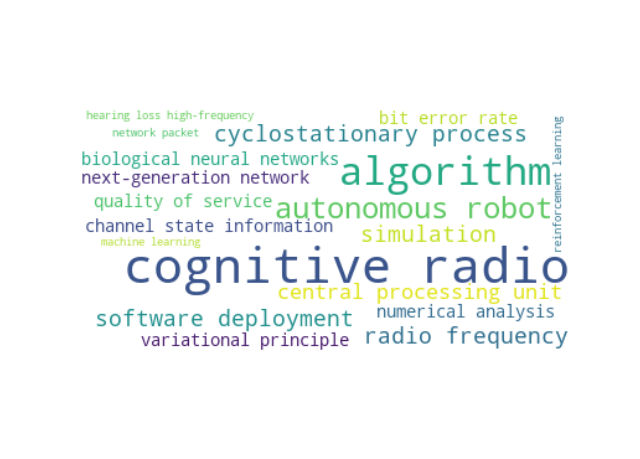
\includegraphics[width=0.495\textwidth]{img/topic2.png}\\
	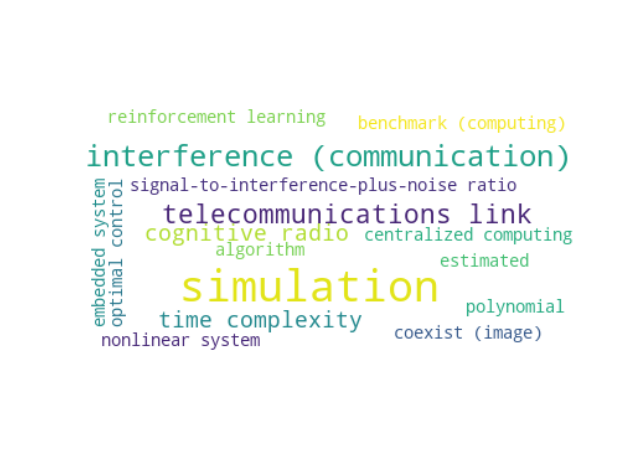
\includegraphics[width=0.495\textwidth]{img/topic3.png}
	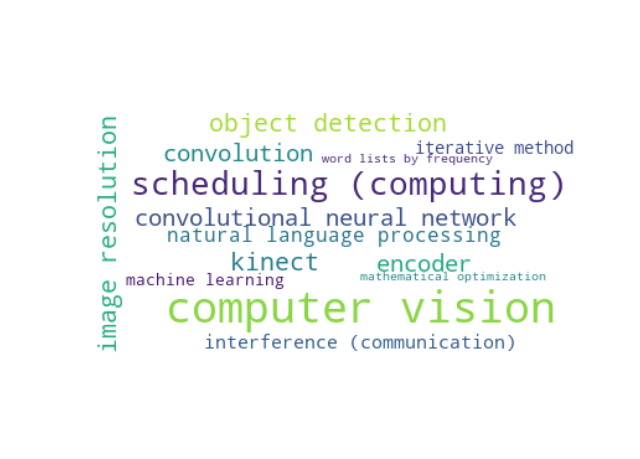
\includegraphics[width=0.495\textwidth]{img/topic4.png}
	\caption{These are some examples of the $K$ time-fused topics, that are computed during \textbf{Task 2}, the frequency of the word in the respective topic-chains is used in order to determine the font-size in the word cloud.}\label{fig:fusedtopics}
\end{figure}

\newpage
\bibliographystyle{unsrt}
\bibliography{ref}



\end{document}
